% !TEX program = tectonic
% Deck AUTONOME « La donnée de la Chambre, de bout en bout » (House 2013-2026).
% Format repris de SLIDES_DONNEES_S1S2_V2.tex : thème Madrid, mécanisme \pipefig (carte
% unique du trajet, une seule étape allumée), \choixbox, \repband, \partdivider.
%
% BUT (demande d'Alice, 2026-07-21) : qu'après lecture on ait VRAIMENT compris la donnée.
% Quatre exigences, qui commandent le plan :
%   (1) chaque chiffre est DÉCOMPOSABLE — aucun total sans ses parties, et la somme boucle ;
%   (2) tous les CHOIX de traitement sont énoncés, chiffrés, avec l'autre option quand elle est mesurée ;
%   (3) ce qui reste INEXPLOITÉ est dit, en lignes / dollars / membres ;
%   (4) ce que la donnée PERMET et NE PERMET PAS pour une stratégie.
%
% SOURCE UNIQUE DES CHIFFRES : 01_v1_house/Portefeuilles_House_Complet.ipynb (158 cellules,
% toutes exécutées). Aucun chiffre de ce deck n'est écrit à la main : chacun sort d'une cellule.
% La fiche FICHE_DONNEES_HOUSE.pdf est le résumé 4 pages du même contenu — mêmes chiffres.
% Figures : ../figures/fig_10_*.png, produites par ce même notebook.
%
% Additif : ne modifie ni le notebook, ni la fiche, ni les autres decks.
\documentclass[11pt,aspectratio=169]{beamer}
\definecolor{helec}{HTML}{3B6EA5}   % couleur maîtresse
\usetheme{Madrid}
\usecolortheme[named=helec]{structure}
\setbeamertemplate{navigation symbols}{}
\setbeamertemplate{blocks}[rounded][shadow=false]
\setbeamerfont{frametitle}{series=\bfseries}
\usepackage[T1]{fontenc}
\usepackage{lmodern}
\usepackage[utf8]{inputenc}
\usepackage[french]{babel}
\usepackage{booktabs}
\usepackage{xcolor}
\usepackage{graphicx}
\usepackage{amssymb}
\usepackage{amsmath}
\usepackage{array}
\usepackage{newunicodechar}
\usepackage{tikz}
\usetikzlibrary{arrows.meta,positioning,calc}
\hypersetup{colorlinks=true, urlcolor=helec, linkcolor=white}
\graphicspath{{../figures/}{figs/}}

% Caractères Unicode → commandes (fontes T1)
\newunicodechar{→}{\ensuremath{\rightarrow}}
\newunicodechar{—}{\textemdash}
\newunicodechar{–}{\textendash}
\newunicodechar{…}{\ldots}
\newunicodechar{·}{\textperiodcentered}
\newunicodechar{≈}{\ensuremath{\approx}}
\newunicodechar{×}{\ensuremath{\times}}
\newunicodechar{≤}{\ensuremath{\leq}}
\newunicodechar{≥}{\ensuremath{\geq}}
\newunicodechar{−}{\ensuremath{-}}
\newunicodechar{±}{\ensuremath{\pm}}
\newunicodechar{✓}{\checkmark}
\newunicodechar{↔}{\ensuremath{\leftrightarrow}}
\newunicodechar{≠}{\ensuremath{\neq}}
\newunicodechar{⊇}{\ensuremath{\supseteq}}
\newunicodechar{⊂}{\ensuremath{\subset}}
\newunicodechar{∑}{\ensuremath{\textstyle\sum}}
\newunicodechar{∧}{\ensuremath{\wedge}}
\newunicodechar{⇒}{\ensuremath{\Rightarrow}}
\newunicodechar{œ}{\oe}
\newunicodechar{Œ}{\OE}
\newunicodechar{°}{\textdegree}
\newunicodechar{§}{\S}
\newunicodechar{«}{\og}
\newunicodechar{»}{\fg{}}

% ── Code couleur ──
% Le deck n'a que deux familles : ce que le MEMBRE dépose (bleu), ce que NOUS en faisons (vert).
% L'ocre marque la donnée intermédiaire, le rouge un choix ou une alerte.
\definecolor{helec}{HTML}{3B6EA5}     % bleu — l'acte I : le membre dépose
\definecolor{hocr}{HTML}{A9C5E2}      % bleu clair — la voie scannée (OCR)
\definecolor{okgreen}{HTML}{2E8B57}   % vert — l'acte II : ce qu'on en fait
\definecolor{alertred}{HTML}{C0392B}
\definecolor{warnorange}{HTML}{E67E22}
\definecolor{dataC}{RGB}{176,110,14}  % ocre — la donnée en transit
\definecolor{grisC}{RGB}{90,90,90}

\newcommand{\co}[1]{\texttt{#1}}
\tikzset{
  step/.style={rectangle, rounded corners=2pt, draw=#1, line width=0.8pt, fill=#1!8,
               align=center, font=\scriptsize, minimum height=0.72cm},
  bande/.style={rectangle, rounded corners=2pt, draw=#1, line width=0.8pt, fill=#1!8,
                align=center, font=\scriptsize, minimum height=0.62cm},
  arr/.style={-{Latex[length=2mm]}, line width=0.8pt, draw=gray!65},
}

\newcommand{\badge}[2]{\colorbox{#1}{\textcolor{white}{\footnotesize\textbf{#2}}}}
\newcommand{\badgel}[2]{\colorbox{#1}{\textcolor{black!80}{\footnotesize\textbf{#2}}}}
\newcommand{\kpi}[3]{{\large\textbf{\textcolor{#1}{#2}}}~{\footnotesize #3}}
\newcommand{\defl}[1]{{\scriptsize\color{black!55}#1}}

% Carreau chiffre-clé : \tuile{couleur}{gros chiffre}{légende}
\newcommand{\tuile}[3]{%
  \begin{minipage}[t]{0.23\textwidth}\centering
    \colorbox{#1}{\parbox[c][20mm][c]{\dimexpr\linewidth-8pt}{\centering
      {\color{white}\Large\textbf{#2}}\\[0.5mm]{\color{white}\footnotesize #3}}}
  \end{minipage}}

% Encadré CHOIX : une décision de traitement, ce qu'elle déplace, ce que l'autre option donnerait.
\newcommand{\choixbox}[1]{%
  \colorbox{alertred!8}{\parbox{\dimexpr\linewidth-8pt}{\scriptsize
    \textbf{\textcolor{alertred}{CHOIX}}\; --- #1}}}
% Bandeau RÉPONSE : la conclusion d'une partie, en une phrase.
\newcommand{\repband}[1]{%
  \colorbox{okgreen!12}{\parbox{\dimexpr\textwidth-10pt}{\scriptsize
    \textbf{\textcolor{okgreen}{Réponse}}\; --- #1}}}
% Bandeau PIÈGE : une confusion à ne pas faire (deux chiffres qui se ressemblent, un mot polysémique).
\newcommand{\piege}[1]{%
  \colorbox{warnorange!12}{\parbox{\dimexpr\linewidth-8pt}{\scriptsize
    \textbf{\textcolor{warnorange}{PIÈGE}}\; --- #1}}}

% Bande maths : \bmaths{noms des termes}{formule sur une ligne}
\newcommand{\bmaths}[2]{%
  {\scriptsize\color{black!55}#1}\\[0.2mm]
  {\small$\displaystyle #2$}\\[2mm]}

% Séparateur de partie plein cadre : \partdivider{couleur}{PARTIE X}{Grand titre}{sous-titre}
\newcommand{\partdivider}[4]{%
  {\setbeamercolor{background canvas}{bg=#1}
  \begin{frame}[plain]
    \centering\vfill
    {\color{white}\Large\textbf{#2}}\\[3.5mm]
    {\color{white!75}\rule{0.40\textwidth}{1pt}}\\[4.5mm]
    {\color{white}\fontsize{32}{36}\selectfont\textbf{#3}}\\[5.5mm]
    {\color{white!88}\large #4}
    \vfill
  \end{frame}}}
% Intercalaire de chapitre : \chapdivider{label}{Grand titre}{sous-titre}
\newcommand{\chapdivider}[3]{%
  \begin{frame}[plain]
    \centering\vfill
    {\color{helec!85}\large\textbf{#1}}\\[3.5mm]
    {\color{black!88}\fontsize{29}{33}\selectfont\textbf{#2}}\\[4mm]
    {\color{helec!45}\rule{0.30\textwidth}{1.2pt}}\\[4mm]
    {\color{black!55}\large #3}
    \vfill
  \end{frame}}

% Ligne d'étape dans un sommaire : \etape{n}{titre}{glose}
\newcommand{\etape}[3]{%
  {\color{helec}\bfseries #1}\; & \textbf{#2} & {\scriptsize\color{black!60} #3}\\[0.6mm]}

% ════════════════════════════════════════════════════════════════════════════════
%  LA CARTE — dessin unique du trajet, réutilisé à chaque étape
% ════════════════════════════════════════════════════════════════════════════════
% \pipefig{k} : k = 0 → tout allumé (vue d'ensemble) ; k = 1..9 → seule l'étape k est allumée,
% le reste est estompé à 16 %. Même dessin à chaque fois, seul le curseur bouge.
%
% Le trajet a deux moitiés, et la carte le montre :
%   ACTE I (bleu, étapes 1-4) — ce que le MEMBRE dépose, dans l'ordre de son mandat :
%       1 il arrive · 2 il trade · 3 il déclare · 4 il part
%   la CHARNIÈRE — les dépôts ne portent pas une matière mais DEUX : des positions
%       (Schedule A : ce qu'il possède) et des transactions (Schedule B : ce qu'il a échangé).
%       Cette séparation commande tout l'aval : les positions donnent le point de départ et
%       servent de juge, les transactions font bouger le portefeuille.
%   ACTE II (vert, étapes 5-9) — ce que NOUS en faisons :
%       5 rassembler · 6 trier · 7 valoriser · 8 reconstruire · 9 vérifier
%
% Correspondance étape → bandes du dessin (les lettres nomment les BANDES, pas les étapes) :
%   1 = \opA (arrivée)      4 = \opD (sortie)        7 = \opG (valoriser)
%   2 = \opB (fil de l'eau) 5 = \opE (rassembler)    8 = \opH (reconstruire)
%   3 = \opC (annuel)       6 = \opF (trier)         9 = \opI (vérifier)
%   \opS = la charnière A/B — allumée en 1, 2, 3, 4 (elle explique ce que chaque dépôt porte)
%          et en vue d'ensemble.
\newcommand{\pipefig}[1]{%
  \def\opA{0.16}\def\opB{0.16}\def\opC{0.16}\def\opD{0.16}\def\opS{0.16}%
  \def\opE{0.16}\def\opF{0.16}\def\opG{0.16}\def\opH{0.16}\def\opI{0.16}%
  \ifnum#1=0 \def\opA{1}\def\opB{1}\def\opC{1}\def\opD{1}\def\opS{1}%
             \def\opE{1}\def\opF{1}\def\opG{1}\def\opH{1}\def\opI{1}\fi
  \ifnum#1=1 \def\opA{1}\def\opS{1}\fi
  \ifnum#1=2 \def\opB{1}\def\opS{1}\fi
  \ifnum#1=3 \def\opC{1}\def\opS{1}\fi
  \ifnum#1=4 \def\opD{1}\def\opS{1}\fi
  \ifnum#1=5 \def\opE{1}\fi  \ifnum#1=6 \def\opF{1}\fi  \ifnum#1=7 \def\opG{1}\fi
  \ifnum#1=8 \def\opH{1}\fi  \ifnum#1=9 \def\opI{1}\fi
  \begin{tikzpicture}[node distance=3mm, every node/.style={transform shape}]
    % ═══ ACTE I — les quatre moments du mandat ═══
    \node[font=\tiny\bfseries, text=helec!80, align=left] at (-8.2,0.75)
      {ACTE I\\le membre\\dépose};
    \begin{scope}[opacity=\opA, text opacity=\opA]
      \node[step=helec, text width=2.9cm] (arr) at (-4.9,0.75)
        {\textbf{1 · IL ARRIVE}\\{\tiny entrée \emph{H} · candidature \emph{C}}};
    \end{scope}
    \begin{scope}[opacity=\opB, text opacity=\opB]
      \node[step=helec, text width=2.9cm] (fil) at (-1.6,0.75)
        {\textbf{2 · IL TRADE}\\{\tiny déclaration rapide \emph{P}}};
    \end{scope}
    \begin{scope}[opacity=\opC, text opacity=\opC]
      \node[step=helec, text width=2.9cm] (ann) at (1.7,0.75)
        {\textbf{3 · IL DÉCLARE}\\{\tiny rapport annuel \emph{O} · \emph{A}}};
    \end{scope}
    \begin{scope}[opacity=\opD, text opacity=\opD]
      \node[step=helec, text width=2.9cm] (sor) at (5.0,0.75)
        {\textbf{4 · IL PART}\\{\tiny sortie \emph{T}}};
    \end{scope}
    % ═══ LA CHARNIÈRE — un dépôt porte deux matières ═══
    % Les pastilles disent quel moment alimente quelle matière : cinq flèches croisées
    % seraient illisibles sur une carte relue dix fois. Les moments 3 et 4 figurent des DEUX
    % côtés — le rapport annuel, l'amendement et la sortie portent les deux sections, alors
    % que l'arrivée (1) ne porte que des positions et la déclaration rapide (2) que des
    % transactions. C'est le point à retenir de la charnière.
    \begin{scope}[opacity=\opS, text opacity=\opS]
      \node[step=dataC, text width=5.9cm] (schA) at (-3.2,-1.15)
        {\textbf{POSITIONS} --- \emph{Schedule A} \;\colorbox{helec!22}{\tiny\textbf{1·3·4}}\\
         {\tiny ce qu'il possède, à une date}};
      \node[step=dataC, text width=5.9cm] (schB) at (3.3,-1.15)
        {\textbf{TRANSACTIONS} --- \emph{Sch. B} \;\colorbox{helec!22}{\tiny\textbf{2·3·4}}\\
         {\tiny ce qu'il a acheté ou vendu}};
      \node[font=\scriptsize, text=black!60, align=center, text width=13.4cm] at (0,-2.15)
        {les positions donnent le \textbf{point de départ} et servent de \textbf{juge}\\
         les transactions \textbf{font bouger} le portefeuille};
    \end{scope}
    % ═══ ACTE II — ce que nous en faisons ═══
    \node[font=\tiny\bfseries, text=okgreen!80, align=left] at (-8.2,-3.9)
      {ACTE II\\ce qu'on\\en fait};
    \begin{scope}[opacity=\opE, text opacity=\opE]
      \node[bande=okgreen, text width=12.2cm] (ras) at (0,-3.05)
        {\textbf{5 · RASSEMBLER} --- réunir tous les dépôts, compter ce qu'ils contiennent};
    \end{scope}
    \begin{scope}[opacity=\opF, text opacity=\opF]
      \node[bande=okgreen, text width=12.2cm] (tri) at (0,-3.85)
        {\textbf{6 · TRIER} --- chaque ligne reçoit sa classe \emph{avant} tout prix :
         action, fonds, monétaire, code de formulaire};
    \end{scope}
    \begin{scope}[opacity=\opG, text opacity=\opG]
      \node[bande=okgreen, text width=12.2cm] (val) at (0,-4.65)
        {\textbf{7 · VALORISER} --- ne garder que les transactions dont on connaît
         le \textbf{prix du jour}};
    \end{scope}
    \begin{scope}[opacity=\opH, text opacity=\opH]
      \node[bande=okgreen, fill=okgreen!16, text width=12.2cm] (rec) at (0,-5.45)
        {\textbf{8 · RECONSTRUIRE} --- la photo devient un portefeuille en \textbf{parts},
         les transactions le font vivre};
    \end{scope}
    \begin{scope}[opacity=\opI, text opacity=\opI]
      \node[bande=helec, fill=helec!16, text width=12.2cm] (ver) at (0,-6.35)
        {\textbf{9 · VÉRIFIER} --- les \textbf{positions} des rapports annuels, qui n'ont
         jamais servi à construire, jugent le portefeuille};
    \end{scope}
    % ═══ les flèches ═══
    % De la rangée des moments vers la charnière : une flèche par moment, verticale et courte.
    % La répartition A / B est portée par les pastilles, pas par des traits croisés.
    \begin{scope}[opacity=0.30]
      \draw[arr] (arr.south) -- ++(0,-0.30);
      \draw[arr] (fil.south) -- ++(0,-0.30);
      \draw[arr] (ann.south) -- ++(0,-0.30);
      \draw[arr] (sor.south) -- ++(0,-0.30);
      \draw[arr] (schA.south) -- (ras.north -| schA.south);
      \draw[arr] (schB.south) -- (ras.north -| schB.south);
      \draw[arr] (ras) -- (tri); \draw[arr] (tri) -- (val);
      \draw[arr] (val) -- (rec); \draw[arr] (rec) -- (ver);
    \end{scope}
  \end{tikzpicture}}

% Slide-repère « vous êtes ici » : \pipeslide{k}{titre}{la question}{ce qu'on en sort}
\newcommand{\pipeslide}[4]{%
  \begin{frame}{#2}
    \centering
    \resizebox{!}{0.63\textheight}{\pipefig{#1}}\\[2mm]
    \colorbox{helec!10}{\parbox{0.94\textwidth}{\centering\footnotesize\vspace{0.5mm}
      \emph{#3}\\[0.8mm]{\scriptsize\color{black!65} ce qu'on en sort : #4}\vspace{0.5mm}}}
  \end{frame}}
% Bandeau réduit : la carte en tête d'une frame de contenu, pour ne jamais perdre le fil.
\newcommand{\pipestrip}[1]{\resizebox{0.86\textwidth}{!}{\pipefig{#1}}}
% Fil d'Ariane fin : les 9 étapes en une bande, l'étape courante allumée (remplace la carte pleine page).
\newcommand{\pipebread}[1]{%
  \begin{center}\begin{tikzpicture}[x=1.30cm, y=0.6cm, font=\tiny, baseline]
  \foreach \k/\lab/\c [count=\i from 0] in {%
    1/il arrive/helec, 2/il trade/helec, 3/il déclare/helec, 4/il part/helec,
    5/on rassemble/okgreen, 6/on trie/okgreen, 7/on valorise/okgreen,
    8/on reconstruit/okgreen, 9/on vérifie/okgreen}{%
    \ifnum\k<9 \draw[\c!35, line width=0.7pt] ({\i+0.17},0) -- ({\i+0.83},0);\fi
    \ifnum\k=#1
      \fill[\c] ({\i},0) circle (0.18);
      \node[text=white, font=\tiny\bfseries] at ({\i},0) {\k};
      \node[text=\c, font=\tiny\bfseries, anchor=north] at ({\i},-0.24) {\lab};
    \else
      \fill[\c!22] ({\i},0) circle (0.12);
      \node[text=\c!60, font=\tiny] at ({\i},0) {\k};
    \fi}
  \end{tikzpicture}\end{center}\vspace{-0.5mm}}

\title[La donnée de la Chambre]{\textbf{La donnée de la Chambre, de bout en bout}}
\subtitle{Ce qu'ils déposent, ce qu'on en fait, ce qu'on peut en tirer}
\author{}
\date{}

\begin{document}

% ═══════════ part0 ═══════════
% ════════════════════════════════════════════════════════════════════════════════
%  PART 0 — OUVERTURE
%  Titre · la question · la carte · le sommaire · le mode d'emploi des chiffres ·
%  les quatre exigences.
%  Tous les chiffres viennent du notebook Portefeuilles_House_Complet (cellules citées).
% ════════════════════════════════════════════════════════════════════════════════

% ── 1 · Page de titre ───────────────────────────────────────────────────────────
\begin{frame}[plain]
  \centering\vfill
  {\color{helec}\fontsize{30}{34}\selectfont\textbf{La donnée de la Chambre,}}\\[1.5mm]
  {\color{helec}\fontsize{30}{34}\selectfont\textbf{de bout en bout}}\\[5mm]
  {\color{helec!45}\rule{0.42\textwidth}{1.2pt}}\\[5mm]
  {\color{black!70}\large Ce qu'ils déposent, ce qu'on en fait, ce qu'on peut en tirer}\\[3mm]
  {\color{black!45}\footnotesize Chambre des représentants · transactions 2013--2026}\\[8mm]
  \colorbox{helec!8}{\parbox{0.84\textwidth}{\centering\footnotesize\vspace{1mm}
    À la fin de ce document, vous saurez d'où vient chacune des \textbf{129\,538} transactions
    reconstituées, ce qui manque à celles qu'on ne reconstruit pas,
    et ce que cette donnée autorise --- ou interdit --- à une stratégie.\vspace{1mm}}}
  \vfill
\end{frame}

% ── 2 · La question ─────────────────────────────────────────────────────────────
\begin{frame}{De quoi dispose-t-on exactement, et que peut-on en faire ?}
  \begin{columns}[T]
    \begin{column}{0.50\textwidth}
      \footnotesize
      Deux questions, dans cet ordre, et jamais mélangées :
      \begin{itemize}\itemsep2.5pt
        \item \textbf{de quoi dispose-t-on ?} --- quels documents un membre dépose,
              ce qu'ils contiennent, ce qu'on arrive à en lire ;
        \item \textbf{que peut-on en faire ?} --- ce qu'on reconstruit avec,
              ce que la reconstruction rate, et ce qui reste hors d'atteinte.
      \end{itemize}
      \vspace{2mm}
      \defl{Ce document décrit la donnée. Il ne juge aucune performance.}
    \end{column}
    \begin{column}{0.46\textwidth}
      \footnotesize\raggedright
      \kpi{helec}{900}{membres au registre}\\
      \defl{toute personne ayant siégé à la Chambre entre 2013 et 2026,
        d'après le référentiel officiel des mandats (couverture 900/900)}\\[2.5mm]
      \kpi{dataC}{609\,886}{lignes de patrimoine déposées}\\
      \defl{dépôts 2014--2026, empilés : le même actif revient à chaque
        déclaration --- ce n'est pas un patrimoine, on le décompose plus loin}\\[2.5mm]
      \kpi{okgreen}{129\,538}{transactions retenues}\\
      \defl{2013--2026 : ce qu'on arrive à rejouer, chez 408 membres}
    \end{column}
  \end{columns}
  \vspace{2.5mm}
  \colorbox{black!5}{\parbox{\dimexpr\textwidth-8pt}{\scriptsize\vspace{0.5mm}
    \textbf{D'où vient tout ce qui suit.} Un seul notebook, toutes cellules exécutées :
    \co{Portefeuilles\_House\_Complet}. Chaque chiffre est recopié d'une sortie de cellule, chaque
    figure produite par ce notebook --- rien n'est estimé ni repris d'un travail antérieur (seules
    quatre tables v1 gelées sont rechargées et recomptées).\vspace{0.5mm}}}
\end{frame}

% ── 3 · La carte d'ensemble ─────────────────────────────────────────────────────
\begin{frame}{Quatre moments de dépôt, deux matières, cinq traitements}
  \centering
  \resizebox{0.80\textwidth}{!}{\pipefig{0}}\\[1mm]
  {\scriptsize\color{black!55} \emph{A} = amendement, la version corrigée d'un dépôt déjà remis
  --- on la retrouve en fil d'Ariane, allumée, en tête de chaque étape}
\end{frame}

% ── 4 · Le sommaire ─────────────────────────────────────────────────────────────
\begin{frame}{Deux actes, neuf étapes}
  \centering\small
  \begin{tabular}{@{}c@{\hspace{2.5mm}}l@{\hspace{3mm}}l@{}}
    \multicolumn{3}{@{}l}{\textcolor{helec}{\footnotesize\textbf{ACTE I — le membre dépose}}}\\[0.6mm]
    \etape{1}{Il arrive}{sa photo d'entrée \emph{H}, ou sa candidature \emph{C} : ce qu'il possède au départ}
    \etape{2}{Il trade}{la déclaration rapide \emph{P}, une transaction à la fois}
    \etape{3}{Il déclare}{le rapport annuel \emph{O}, ou son amendement \emph{A} :
      ses positions \emph{et} ses transactions de l'année}
    \etape{4}{Il part}{sa photo de sortie \emph{T} : le dernier état connu}
    \multicolumn{3}{@{}l}{\parbox{0.95\textwidth}{\raggedright
      \hspace{1mm}\textcolor{dataC}{\scriptsize\textbf{la charnière}} \;
      {\scriptsize\color{black!60} un formulaire de patrimoine a deux sections : des
      \emph{positions} (Schedule A) et des \emph{transactions} (Schedule B). La déclaration
      rapide \emph{P} ne porte que des transactions ; \emph{H} et \emph{C} que des positions ;
      \emph{O}, \emph{A} et \emph{T} portent les deux.}}}\\[0.4mm]
    \multicolumn{3}{@{}l}{\textcolor{okgreen}{\footnotesize\textbf{ACTE II — ce qu'on en fait}}}\\[0.6mm]
    \etape{5}{On rassemble}{réunir le flux électronique et les documents scannés, et compter}
    \etape{6}{On trie}{chaque ligne reçoit sa classe --- action, fonds, monétaire, code de
      formulaire --- \emph{avant} tout prix}
    \etape{7}{On valorise}{ne garder que ce dont on connaît le prix du jour}
    \etape{8}{On reconstruit}{\parbox[t]{0.72\textwidth}{\raggedright la photo devient un
      portefeuille en \emph{parts} --- une valeur de part qui démarre à 1, comme un fonds ---
      et les transactions le font vivre}}
    \etape{9}{On vérifie}{\parbox[t]{0.72\textwidth}{\raggedright les \emph{positions} des rapports
      annuels (Schedule A), jamais utilisées pour construire, jugent le portefeuille reconstruit ;
      leurs \emph{transactions} (Schedule B), elles, ont servi à le construire}}
  \end{tabular}\\[0.2mm]
  {\scriptsize\color{black!60} Puis trois parties : \textbf{les choix qu'on a faits} (chaque
  décision, son volume, l'autre option), \textbf{ce qui reste} (l'inexploité, le fragile,
  l'inexistant), \textbf{ce qu'on peut en faire}.}
\end{frame}

% ── 5 · Le mode d'emploi des chiffres ───────────────────────────────────────────

% ── 6 · Les quatre exigences ────────────────────────────────────────────────────

% ═══════════ part1 ═══════════
% ════════════════════════════════════════════════════════════════════════════════
%  ACTE I — ce que le membre dépose, dans l'ordre de son mandat
% ════════════════════════════════════════════════════════════════════════════════
\partdivider{helec}{ACTE I}{Ce qu'ils déposent}{la vie d'un mandat, dans l'ordre}

% ── LA POPULATION ───────────────────────────────────────────────────────────────
\begin{frame}{Le socle de tout le deck : 900 membres, quatre trajectoires}
  \centering
  \begin{tabular}{@{}r@{\;}cc@{}}
    & {\footnotesize\emph{déjà là en 2014} \; \textbf{439}}
    & {\footnotesize\emph{arrivé après 2014} \; \textbf{461}}\\[1mm]
    {\footnotesize\emph{encore en poste} \; \textbf{437}} &
    \colorbox{helec!16}{\parbox[c][13mm][c]{0.34\textwidth}{\centering
      {\Large\textbf{125}}\\[0.4mm]{\footnotesize déjà-là restés}}} &
    \colorbox{okgreen!16}{\parbox[c][13mm][c]{0.34\textwidth}{\centering
      {\Large\textbf{312}}\\[0.4mm]{\footnotesize arrivés restés}}}\\[1.6mm]
    {\footnotesize\emph{parti avant 2026} \; \textbf{463}} &
    \colorbox{helec!8}{\parbox[c][13mm][c]{0.34\textwidth}{\centering
      {\Large\textbf{314}}\\[0.4mm]{\footnotesize déjà-là partis}}} &
    \colorbox{okgreen!8}{\parbox[c][13mm][c]{0.34\textwidth}{\centering
      {\Large\textbf{149}}\\[0.4mm]{\footnotesize cycle complet}}}\\
  \end{tabular}\\[2mm]
  \defl{chaque membre est dans une case et une seule --- était-il en poste au 1\textsuperscript{er} janvier
  2014, l'est-il encore au 1\textsuperscript{er} janvier 2026 ? \quad 125 + 314 + 312 + 149 = \textbf{900}.
  \; Le registre des membres est cadré 2014-2026 ; les transactions, elles, sont cadrées 2013-2026.}\\[3.5mm]
  \kpi{helec}{900}{membres au registre}\qquad
  \kpi{helec}{98,9 \%}{de concordance avec les mandats officiels}\qquad
  \kpi{alertred}{18}{sans document}\\[2mm]
  \defl{98,9 \% = 890 des 900 membres tombent dans la même case selon nos dépôts et selon le
  référentiel officiel des mandats ; les 10 désaccords sont des cas de frontière, listés nommément
  \quad·\quad les 18 sans document : 10 déjà-là partis, 5 arrivés restés,
  2 déjà-là restés, 1 cycle complet}
\end{frame}

\begin{frame}{Sur 900 membres, 408 ont une transaction qu'on sait rejouer}
  \centering
  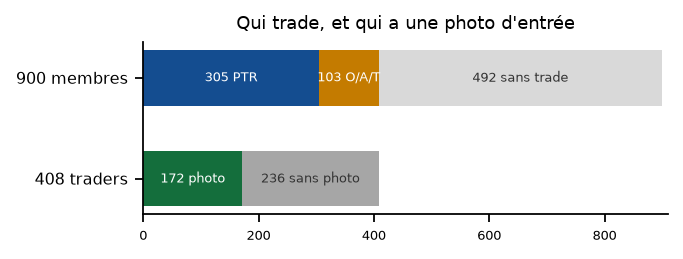
\includegraphics[width=0.58\textwidth]{fig_10_partition.png}\\[0.5mm]
  {\scriptsize\color{black!60} sur la figure : « PTR » = déclaration rapide · « O/A/T » = rapport
  annuel \emph{O} + amendement \emph{A} + sortie \emph{T}.}\\[1.5mm]
  \begin{columns}[t]
    \begin{column}{0.50\textwidth}\footnotesize
      \textbf{Par quel canal on les voit}\\[0.8mm]
      \begin{tabular}{@{}rl@{}}
        \textbf{305} & vus par les déclarations rapides\\
        \textbf{103} & vus seulement par les rapports annuels\\
        \textbf{492} & aucune transaction qu'on sache rejouer\\
        \midrule
        \textbf{900} & membres du registre\\
      \end{tabular}
    \end{column}
    \begin{column}{0.46\textwidth}\footnotesize
      \textbf{Les 408 qui tradent, au départ}\\[0.8mm]
      \begin{tabular}{@{}rl@{}}
        \textbf{172} & ont une photo d'entrée exploitable\\
        \textbf{236} & n'en ont pas : patrimoine nul au départ\\
        \midrule
        \textbf{408} & membres qui tradent\\
      \end{tabular}
    \end{column}
  \end{columns}\vspace{1.5mm}\par
  \defl{« 492 » ne dit pas « ne trade pas » : 315 membres ont des lignes de déclaration rapide,
  305 survivent au filtre des cours.}
\end{frame}

\begin{frame}{Quatre documents, et une information qui vieillit de 27 jours à plus d'un an}
  \centering
  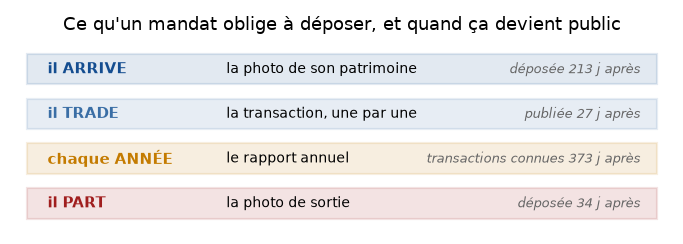
\includegraphics[width=0.74\textwidth]{fig_10_obligations.png}\\[2mm]
  \defl{médianes sur nos dépôts (pas des délais légaux) : \textbf{213 j} après l'entrée · \textbf{27 j}
  et \textbf{373 j} après l'opération · \textbf{34 j} après la fin du mandat.}\\[2mm]
  \piege{le rapport annuel n'est pas une redite tardive sans intérêt : c'est le seul canal qui
  voit 103 des 408 membres qui tradent. Mais son information a plus d'un an quand elle devient publique.}
\end{frame}

% ── 1 · IL ARRIVE ───────────────────────────────────────────────────────────────
\begin{frame}{À l'arrivée : 319 des 461 arrivants déposent leur photo}
  \pipebread{1}
  \centering
  
\includegraphics[width=0.39\textwidth]{fig_10_etape_arrivee.png}\\[1mm]
  \begin{columns}[t]
    \begin{column}{0.52\textwidth}\footnotesize
      \textbf{D'où sortent les 325 photos}\\[0.8mm]
      \begin{tabular}{@{}rl@{}}
        \textbf{378} & documents d'entrée \emph{H} au corpus\\
        \textbf{7\,670} & candidatures \emph{C} au corpus\\
        \textbf{291} & membres re-sélectionnés (dont 52 par un \emph{C})\\
        \textbf{+34} & gardés de la sélection précédente\\
        \midrule
        \textbf{325} & photos d'entrée retenues, une par membre\\
      \end{tabular}\\[1mm]
      \defl{règle : le \emph{H} s'il existe, sinon le \emph{C} le plus proche du début de mandat,
      cherché dans les deux sources · 34 photos conservées de la sélection précédente.}
    \end{column}
    \begin{column}{0.44\textwidth}\footnotesize
      \textbf{Attendu contre observé}\\[0.8mm]
      \begin{tabular}{@{}rl@{}}
        \textbf{461} & membres devaient en déposer une\\
        \textbf{319} & l'ont fait \; \textrightarrow{} \; \textbf{142} manquantes\\
        \textbf{+6} & photos chez des non-attendus\\
        \midrule
        \textbf{325} & photos d'entrée en main\\
      \end{tabular}\\[1.2mm]
      \defl{461 attendues = 312 arrivés restés + 149 cycles complets.}\\[2mm]
      \kpi{warnorange}{213 jours}{de délai médian entre l'entrée en mandat et le dépôt (n = 258)}
    \end{column}
  \end{columns}
\end{frame}

% ── 2 · IL TRADE ────────────────────────────────────────────────────────────────
\begin{frame}{La déclaration rapide est le seul document exploité à 100 \%}
  \pipebread{2}
  \footnotesize
  \begin{columns}[t]
    \begin{column}{0.50\textwidth}
      \textbf{Ce que le canal rapide apporte}\\[1.2mm]
      \begin{tabular}{@{}rl@{}}
        \textbf{5\,571} & dépôts (membre × date de divulgation)\\
        \textbf{122\,814} & lignes de transactions, Chambre\\
        \textbf{315} & membres concernés\\
        \textbf{4\,340} & tickers distincts\\
      \end{tabular}
    \end{column}
    \begin{column}{0.46\textwidth}
      \kpi{okgreen}{100 \%}{des 8\,267 documents \emph{P} du journal sont exploités}\\[2mm]
      \defl{aucun autre document n'atteint ce taux : les photos du patrimoine en perdent de 25 à 60 \%
      (partie IV).}\\[3mm]
      \kpi{warnorange}{27 jours}{de délai médian entre l'opération et sa publication (q90 : 49 j)}
    \end{column}
  \end{columns}
\end{frame}

% ── 3 · IL DÉCLARE ──────────────────────────────────────────────────────────────
\begin{frame}{Le membre médian a 85 \% de ses années de mandat couvertes}
  \pipebread{3}
  \centering
  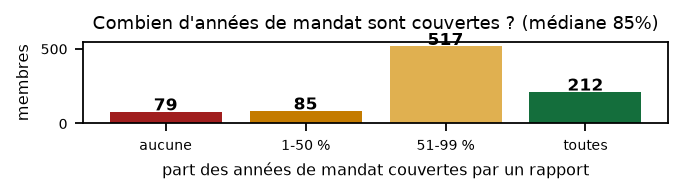
\includegraphics[width=0.36\textwidth]{fig_10_etape_annuel.png}\\[1mm]
  \begin{columns}[t]
    \begin{column}{0.50\textwidth}\footnotesize
      \textbf{Combien de rapports sont dus}\\[0.8mm]
      \begin{tabular}{@{}rl@{}}
        \textbf{5\,702} & rapports annuels attendus, 2013-2025\\
        \textbf{7} & membres n'en doivent aucun\\
        \textbf{893} & membres en doivent au moins un\\
        \textbf{814} & membres en ont déposé au moins un\\
      \end{tabular}\\[1mm]
      \defl{un rapport déposé en Y couvre Y$-$1 ; il est dû pour toute année en mandat au 31/12.
      La mesure porte sur \emph{chaque membre} : les 5\,702 années dues ne sont pas confrontées
      à un total observé.}
    \end{column}
    \begin{column}{0.46\textwidth}\footnotesize
      \textbf{Taux de couverture médian, par trajectoire}\\[0.8mm]
      \begin{tabular}{@{}lr@{}}
        cycle complet & 100 \%\\
        déjà-là restés & 92 \%\\
        arrivés restés & 86 \%\\
        déjà-là partis & 83 \%\\
        \midrule
        \textbf{médiane, 893 membres} & \textbf{85 \%}\\
      \end{tabular}\\[1mm]
      \defl{les barres de la figure comptent des \emph{membres}, pas des années.}
    \end{column}
  \end{columns}\vspace{1mm}\par
  \defl{ne pas trader n'est pas ne pas déclarer : sur les \textbf{509} membres qu'on ne voit jamais
  trader, \textbf{444} (87 \%) déposent quand même leurs rapports.}
\end{frame}

% ── 4 · IL PART ─────────────────────────────────────────────────────────────────
\begin{frame}{À la sortie : 367 des 463 partants déposent, 96 manquent}
  \pipebread{4}
  \centering
  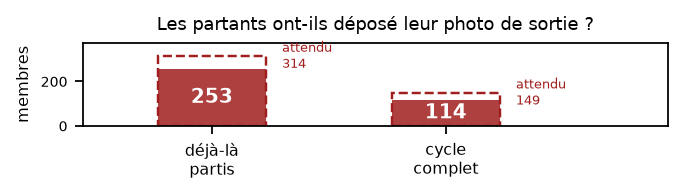
\includegraphics[width=0.44\textwidth]{fig_10_etape_sortie.png}\\[1mm]
  \begin{columns}[t]
    \begin{column}{0.50\textwidth}\footnotesize
      \textbf{Attendu contre observé}\\[0.8mm]
      \begin{tabular}{@{}rl@{}}
        \textbf{463} & membres devaient en déposer une\\
        \textbf{367} & l'ont fait \; \textrightarrow{} \; \textbf{96} manquantes\\
        \textbf{+7} & photos chez des membres restés\\
        \midrule
        \textbf{374} & membres avec photo de sortie\\
      \end{tabular}\\[1mm]
      \defl{463 attendues = 314 déjà-là partis + 149 cycles complets.}
    \end{column}
    \begin{column}{0.46\textwidth}\footnotesize
      \kpi{warnorange}{34 jours}{de délai médian entre la fin du mandat et le dépôt (n = 374)}\\[2.5mm]
      \textbf{La sortie porte aussi des mouvements}\\[0.8mm]
      \begin{tabular}{@{}rl@{}}
        \textbf{21\,175} & lignes de positions (379 documents)\\
        \textbf{9\,900} & lignes de transactions (157 documents)\\
      \end{tabular}\\[1mm]
      \defl{la sortie porte aussi des transactions : elles nourrissent le flux (étape 7).}
    \end{column}
  \end{columns}\vspace{1.5mm}\par
  \defl{la photo de sortie ne sert jamais à construire le portefeuille : elle est réservée
  au rôle de juge (acte II, étape 9).}
\end{frame}

% ── LA CHARNIÈRE A / B ──────────────────────────────────────────────────────────
\begin{frame}{Deux sections dans le formulaire, et elles ne servent pas à la même chose}
  \begin{columns}[c]
    \begin{column}{0.54\textwidth}
      \centering
      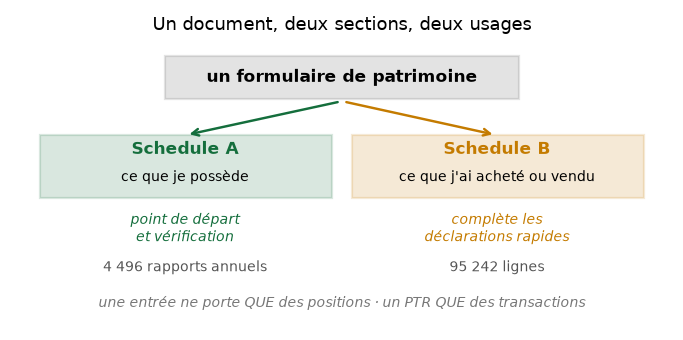
\includegraphics[width=\textwidth]{fig_10_deux_sections.png}\\[1mm]
      {\scriptsize\color{black!60} les deux chiffres portés sur la figure sont ceux du seul
      \emph{rapport annuel O} : 4\,496 documents de positions, 95\,242 lignes de transactions.
      Les totaux de section sont au tableau suivant.}
    \end{column}
    \begin{column}{0.44\textwidth}\footnotesize
      \textbf{\textcolor{okgreen}{Schedule A --- les positions}}\\
      ce qu'il \emph{possède}, à une date.\\
      \defl{donne le point de départ du portefeuille, et sert de juge à la fin.}\\[3mm]
      \textbf{\textcolor{warnorange}{Schedule B --- les transactions}}\\
      ce qu'il a \emph{acheté ou vendu}.\\
      \defl{fait bouger le portefeuille ; complète les déclarations rapides.}\\[3mm]
      \piege{« déclaration » ne dit rien : il faut toujours préciser \emph{quelle section}.
      La déclaration rapide \emph{P} ne porte que des transactions. L'entrée \emph{H} et la
      candidature \emph{C} ne portent que des positions. Le rapport annuel \emph{O}, l'amendement
      \emph{A} et la sortie \emph{T} portent les deux.}
    \end{column}
  \end{columns}
\end{frame}

\begin{frame}{76 \% du Schedule B est déjà dit par une déclaration rapide}
  \centering
  \vspace{2mm}
  \begin{tabular}{@{}rl@{}}
    \toprule
    \textbf{110\,147} & lignes de Schedule B \; \defl{(95\,242 \emph{O} + 9\,900 \emph{T} + 5\,005 \emph{A})}\\
    $-$ \textbf{84\,032} & déjà dites par une déclaration rapide \; \defl{(76 \% de redite)}\\
    \midrule
    = \textbf{26\,115} & transactions inédites --- le gisement réel des rapports\\
    \bottomrule
  \end{tabular}\\[4mm]
  \piege{deux comptes de lignes de déclarations rapides coexistent, et il faut dire lequel on
  compte : \textbf{56\,002} lignes extraites du corpus de documents --- c'est le compte à périmètre
  égal avec les 110\,147 ci-dessus --- et \textbf{122\,814} lignes dans la table de collecte
  S1/S2, plus complète, qui est la source réelle du flux construit à l'acte II.}\\[3mm]
  \choixbox{« déjà dite » est une règle, pas une évidence : une transaction du rapport est jugée
  connue si une déclaration rapide du même membre porte le même couple (titre, sens) à moins de
  \textbf{365 jours}. Cette seule constante décide du volume d'apport des rapports annuels ---
  aucune autre valeur n'a été mesurée (partie III).}
\end{frame}

% ═══════════ part2 ═══════════
% ══════════════════════════════════════════════════════════════════════════════
%  PART 2 — ACTE II (1) : 5 on rassemble · 6 on trie · 7 on valorise
% ══════════════════════════════════════════════════════════════════════════════

\partdivider{okgreen}{ACTE II}{Ce qu'on en fait}{de la ligne déclarée au portefeuille}

% ───────────────────────────────── ÉTAPE 5 ────────────────────────────────────

\begin{frame}{L'océrisation était payée et n'était pas branchée : +188\,970 lignes}
  \pipebread{5}
  \footnotesize
  Les positions ne venaient que des dépôts \textbf{électroniques}. Les documents \textbf{scannés}
  étaient déjà océrisés, mais dormants. Les brancher ajoute \textbf{un tiers du patrimoine}.
  \medskip

  \centering
  \begin{tabular}{l r r r}
    \toprule
    voie & documents & lignes & dont tickérisées \\
    \midrule
    dépôt électronique & 12\,459 & 420\,916 & 190\,758 \\
    document scanné, océrisé & 2\,428 & 188\,970 & \;\,81\,535 \\
    \midrule
    \textbf{table fusionnée} & \textbf{14\,887} & \textbf{609\,886} & \textbf{272\,293} \\
    \bottomrule
  \end{tabular}\\[4mm]

  \raggedright
  \choixbox{on accepte cet OCR : \textbf{0} document commun aux deux voies, \textbf{66 \%} des lignes
  océrisées portent une fourchette conforme à la grille. \defl{Contrôles complets et option « électronique seul » au notebook.}}
\end{frame}

% ───────────────────────────────── ÉTAPE 6 ────────────────────────────────────
\begin{frame}{On classe l'actif avant de connaître son prix}
  \pipebread{6}
  \footnotesize
  \textbf{La règle d'or} : chaque ligne reçoit sa classe d'après son \emph{libellé}, \emph{avant}
  toute recherche de prix. Le moteur ne voit ensuite que la classe \textbf{négociable} (action ou ETF).
  \medskip

  \centering
  Exemple sur les 26\,115 transactions de rapports annuels que les déclarations rapides
  n'avaient pas déjà dites :\\[1.5mm]
  \begin{tabular}{l r l}
    \toprule
    classe & lignes & décidée par \\
    \midrule
    négociable \defl{(action, ETF)} & 16\,062 & \defl{ticker reconnu, libellé d'actif} \\
    fonds mutuel                    & 9\,393  & \defl{ex. 5 lettres finissant par X} \\
    monétaire                       & 364    & \defl{7 codes listés (SPAXX, FDRXX, VMFXX\ldots)} \\
    faux ticker                     & 296    & \defl{19 codes de formulaire, 5 tickers ambigus bloqués} \\
    \midrule
    \textbf{total} & \textbf{26\,115} & \\
    \bottomrule
  \end{tabular}\\[2mm]

  \raggedright
  \piege{l'ancien moteur gardait « ce qui a un prix » --- or un fonds a une valeur liquidative :
    \textbf{7\,709} lignes de fonds (486~M\$) entraient ainsi dans le moteur \emph{actions}.}
\end{frame}

\begin{frame}{Sur 104\,130~M\$ déclarés, 12\,790 sont des actions --- et c'est un cumul de 13 ans}
  \centering
  
\includegraphics[width=0.50\textwidth]{fig_10_paysage.png}\\[0.5mm]
  {\scriptsize 609\,886 lignes $=$ \textbf{231\,426} actions/ETF (\textbf{12\,790~M\$}) $+$ 337\,593
  sans ticker (87\,405~M\$) $+$ 38\,885 fonds $+$ 1\,106 monétaires $+$ 876 faux tickers ; total
  déclaré \textbf{104\,130~M\$}}\\[1.5mm]
  \begin{columns}[c]
    \begin{column}{0.49\textwidth}\centering
      \colorbox{alertred!8}{\parbox{\dimexpr\linewidth-8pt}{\centering\vspace{0.8mm}
        \scriptsize\textbf{\textcolor{alertred}{PAS « le patrimoine »}}\\[0.6mm]
        {\large\textbf{104\,130~M\$}} · 609\,886 lignes empilées 2014-2026\vspace{0.8mm}}}
    \end{column}
    \begin{column}{0.49\textwidth}\centering
      \colorbox{okgreen!10}{\parbox{\dimexpr\linewidth-8pt}{\centering\vspace{0.8mm}
        \scriptsize\textbf{\textcolor{okgreen}{le stock, à une date}}\\[0.6mm]
        {\large\textbf{8\,887~M\$}} · 42\,522 lignes, 887 déposants --- \textbf{12$\times$ moins}\vspace{0.8mm}}}
    \end{column}
  \end{columns}\vspace{1.5mm}

  \raggedright
  \piege{le même actif est \textbf{recompté à chaque rapport annuel} : la somme des lignes déposées
  n'est pas un patrimoine, c'est un cumul. Le seul chiffre « combien possèdent-ils ? » est
  \textbf{8\,887~M\$}. \defl{Les 337\,593 sans ticker (immobilier, sociétés, comptes) ne sont pas des erreurs --- tri en partie IV.}}
\end{frame}

% ───────────────────────────────── ÉTAPE 7 ────────────────────────────────────

% ── étape 7 : on valorise — 3 cascades + flux F fondus en 1 (détail des entonnoirs → notebook) ──
\begin{frame}{On ne garde que ce qui a un cours : 129\,538 trades, trois sources}
  \pipebread{7}
  \centering\vspace{2mm}
  \kpi{helec}{107\,976}{déclarations rapides} \; $+$ \; \kpi{okgreen}{14\,084}{rapports électroniques}
  \; $+$ \; \kpi{dataC}{7\,478}{Schedule B scanné}\\[3mm]
  {\large\textbf{\textcolor{alertred}{$=$ 129\,538}}}~{\footnotesize transactions valorisées, chez \textbf{408} membres}\\[6mm]
  {\footnotesize Une transaction n'entre que si son titre a un \textbf{cours à la date de
  l'opération}. Ce seul filtre écarte \textbf{14\,833} lignes du fil de l'eau --- \textbf{1\,234}
  tickers sans cours, MMC / FI / WBA en tête.}\\[4mm]
  \choixbox{le Schedule B scanné n'a pas de fourchette de montant lisible : ses 7\,478 trades entrent
  tous au \textbf{forfait de 8\,000,5\,\$}. \defl{Le détail filtre à filtre des trois entonnoirs vit au notebook.}}
\end{frame}

% ═══════════ part3 ═══════════
% ══════════════════════════════════════════════════════════════════════════════
%  PART 3 — ACTE II (2) : 8 on reconstruit · 9 on vérifie
%  Source unique des chiffres : Portefeuilles_House_Complet.ipynb (cellules citées en commentaire).
% ══════════════════════════════════════════════════════════════════════════════

% ── 8.1 le principe (cell 79 MD, cell 88 code) ────────────────────────────────
\begin{frame}{Le portefeuille reconstruit : un compte de \emph{parts}, pas de dollars}
  \pipebread{8}
  \centering\vspace{1mm}
  \bmaths{point de départ — valeur déclarée / prix du jour du dépôt}
         {h_{0,i} \;=\; \tilde v_i \,/\, P_i\!\left(\tau(f_0)\right)}
  \bmaths{achat, puis vente — on ne vend que ce qu'on détient}
         {h_i \;\mathrel{+}=\; \tilde v / P_i(\tau(t)) \qquad\qquad h_i \;\mathrel{-}=\; \min(q_i,\,h_i)}
  \bmaths{valeur, puis rendement du jour — sur les parts de la \textbf{veille}}
         {V(\tau)=\!\textstyle\sum_i h_i(\tau)P_i(\tau) \qquad
          r(\tau)=\frac{\sum_i h_i(\tau-1)P_i(\tau)}{\sum_i h_i(\tau-1)P_i(\tau-1)}-1}
  \defl{$\tilde v$ = milieu de fourchette · $P_i$ = cours de clôture · $\tau(d)$ = 1\up{er} jour coté
  $\geq d$ · $f_0$ = date de \textbf{dépôt} · $t$ = date d'\textbf{opération} · rendement écrêté à $\pm$50~\%}\\[4mm]
  \piege{le rendement se calcule sur les parts de la \textbf{veille} : un apport --- la photo, ou un
  achat --- ne crée jamais de performance (mesuré à l'étape 9). Cette suite de rendements quotidiens,
  un par membre et par jour de bourse, \textbf{est} le portefeuille reconstruit.}
\end{frame}

% ── 8.2 le cas réel (cell 82) ─────────────────────────────────────────────────

% ── 8.3 photo fait foi (cells 87, 94, 65, 80) ─────────────────────────────────
\begin{frame}{La photo fait foi : 11\,277 trades ne sont plus rejoués}
  \small
  Une photo d'entrée déclare l'état \textbf{complet} du patrimoine à sa date. Rejouer un achat
  \emph{antérieur} le compterait deux fois.\\[4mm]
  \centering
  \kpi{alertred}{11\,277}{trades écartés} \quad
  \kpi{alertred}{697 M\$}{de montants} \quad
  \kpi{alertred}{88}{membres}\\[5mm]
  \raggedright
  \choixbox{\co{PHOTO\_FAIT\_FOI = True} : sans cette règle, ces 11\,277 trades étaient rejoués
  \emph{par-dessus} la photo qui les déclare déjà --- double comptage. \defl{« Sa date » = la date de
  \textbf{dépôt}, en médiane 213 j après l'entrée : point de départ jouable, mais tardif.}}
\end{frame}

% ── 8.4 la cascade des photos (cells 83, 80 ; fig_10_entonnoir_h0) ────────────
\begin{frame}{De 325 photos d'entrée retenues à 166 portefeuilles injectés}
  \centering
  
\includegraphics[width=0.78\textwidth]{fig_10_entonnoir_h0.png}\\[0.5mm]
  {\scriptsize
  325 \textbf{retenues}, une par membre (la figure dit \og{}déposées\fg{})
  $-$ \textbf{64} sans ligne négociable valorisée
  $=$ \textbf{261} portant au moins une action valorisée
  $-$ \textbf{18} sans prix au 1\up{er} jour coté $=$ \textbf{243} initialisables
  $=$ \textbf{166} injectées $+$ \textbf{77} sans trade à simuler}\\[1mm]
  \raggedright\scriptsize
  \textbf{Pourquoi on en perd à chaque marche.}
  \begin{itemize}\itemsep0pt\parskip0pt
    \item les \textbf{64} : la photo ne porte que du non coté, des fonds ou des libellés de compte --- rien à valoriser en actions ;
    \item les \textbf{18} : le titre existe, mais aucune série de cours ne commence avant le jour du dépôt ;
    \item les \textbf{77} : le portefeuille de départ est construit, mais le membre n'a aucune transaction à lui appliquer.
  \end{itemize}
  \vspace{0.5mm}
  \centering
  \kpi{okgreen}{7\,782}{lignes (membre, ticker) converties en parts} \quad
  \kpi{okgreen}{84,5 \%}{de la valeur \emph{négociable} des photos (595 M\$)}\\[0.5mm]
  \defl{7\,782 des 8\,860 lignes (membre, ticker) négociables vues en partie I --- les 1\,080 autres
  n'ont pas de cours au jour du dépôt}
\end{frame}

% ── 8.5 partir de zéro (cells 46, 83, 93 ; fig_10_troncature) ─────────────────

% ── 8.6 les quatre reconstructions (cells 89-93) ──────────────────────────────

% ── 8.7 la troncature des ventes (cells 89-93, 100 ; fig_10_troncature) ───────

% ── 9.1 le principe (cells 88, 101 MD, 102, 109) ──────────────────────────────
\begin{frame}{Aucune position qui juge n'a servi à construire}
  \pipebread{9}
  \small
  \begin{columns}[T]
    \begin{column}{0.48\textwidth}
      \badge{okgreen}{CE QUI CONSTRUIT}\\[1.5mm]
      \begin{itemize}\itemsep2pt
        \item \textbf{une seule} photo de positions par membre : la photo d'\textbf{entrée} (H ou C) ;
        \item les \textbf{transactions} : déclarations rapides \textbf{P}, et Schedule B des
              rapports annuels \textbf{O}, des amendements \textbf{A} et des photos de sortie
              \textbf{T} --- en abrégé, O/A/T.
      \end{itemize}
    \end{column}
    \begin{column}{0.48\textwidth}
      \badge{helec}{CE QUI JUGE}\\[1.5mm]
      \begin{itemize}\itemsep2pt
        \item les \textbf{positions} déclarées dans les rapports annuels \textbf{O} (Schedule A) ;
        \item les \textbf{positions} de la photo de \textbf{sortie T}.
      \end{itemize}
    \end{column}
  \end{columns}
  \vspace{3mm}
  \centering
  \repband{Aucune position d'un rapport annuel ni d'une photo de sortie n'entre jamais dans le
  portefeuille. Le seul stock injecté est la photo d'entrée. C'est ce qui rend la mesure honnête :
  le juge n'a pas dicté sa réponse.}\\[2mm]
  \raggedright
  \piege{le même dépôt a deux sections qui ne se recouvrent pas : la \textbf{B} (transactions)
  nourrit le flux, la \textbf{A} (positions) juge. Idem pour la sortie \textbf{T}. Ce qui n'a jamais
  construit, ce sont les \emph{positions}, pas les documents.}
\end{frame}

% ── 9.2 le juge filtré (cells 102, 104) ───────────────────────────────────────

\begin{frame}{Le dossier complet fait passer le rappel médian de 9 \% à 57 \%}
  \centering
  \kpi{helec}{2\,263}{rapports jugent} \quad \kpi{helec}{3\,435}{confrontations}
  \defl{(1\,557 pour les rapides seules · 1\,878 pour le dossier complet)}\\[1mm]
  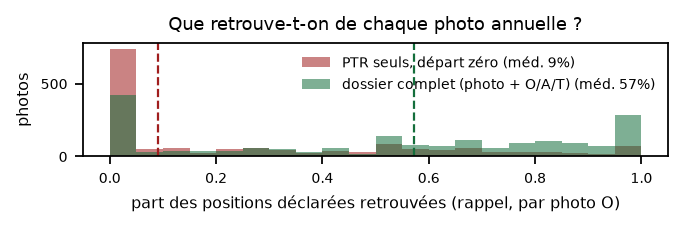
\includegraphics[width=0.54\textwidth]{fig_10_verif_dist.png}\\[1mm]
  \scriptsize
  \begin{tabular}{lrrl}
    \toprule
    médiane par photo & rapides seules & dossier complet & \\
    \midrule
    rappel --- positions retrouvées   & 9 \%  & \textbf{57 \%} & le saut\\
    précision --- positions justes    & 55 \% & 56 \%          & stable\\
    valeurs dans la fourchette         & 44 \% & 47 \%          & à peine\\
    \bottomrule
  \end{tabular}\\[2mm]
  \defl{rappel = communes / déclarées · précision = communes / reconstruites. Un \textbf{second juge},
  la photo de sortie \emph{T} (136 confrontations), donne un rappel médian de \textbf{60 \%}.}
\end{frame}

% ── 9.7 les limites de la vérification (cells 105, 112 MD) ────────────────────
\begin{frame}{Ce que cette vérification ne prouve pas}
  \small
  \begin{itemize}\itemsep4pt
    \item elle ne juge que des \textbf{titres cotés} : immobilier, parts de société, notes sont
          hors du jeu, des deux côtés ;
    \item la mesure de valeur est \textbf{indulgente} : les fourchettes déclarées sont larges, et
          pourtant seules \textbf{47 \%} des positions communes y tombent ;
    \item la photo décrit le \textbf{31 décembre} mais est confrontée au \textbf{jour du dépôt} :
          ce qui a bougé entre les deux compte contre la reconstruction.
  \end{itemize}
  \vspace{2mm}
  \piege{Même dans la meilleure configuration, sur la photo médiane, \textbf{43 \%} des positions
  déclarées ne sont pas reconstruites et \textbf{44 \%} des positions reconstruites ne sont pas
  déclarées. Le dossier complet réduit l'écart ; il ne le ferme pas.}
\end{frame}

% ── 9.8 la réponse de l'acte II ───────────────────────────────────────────────
\begin{frame}{La reconstruction est mesurée, pas décrétée}
  \centering\vspace{2mm}
  \tuile{okgreen}{166}{portefeuilles partis\\ d'une photo réelle}
  \tuile{okgreen}{376}{membres reconstruits,\\ dossier complet}
  \tuile{helec}{3\,435}{confrontations\\ avec un juge}
  \tuile{helec}{57 \%}{rappel médian,\\ dossier complet}\\[6mm]
  \repband{Un compte de parts, parti d'une photo datée quand elle existe (166 cas sur 408) et de
  zéro sinon, jugé par des \textbf{positions déclarées qui n'ont jamais servi à le construire}. Il
  retrouve \textbf{57 \%} de la photo médiane, contre 9 \% sans les rapports annuels. Cinq recomptes
  indépendants (écarts $10^{-9}$ à $10^{-15}$) confirment le calcul.}
\end{frame}

% ═══════════ part4 ═══════════
% ════════════════════════════════════════════════════════════════════════════════
%  PARTIE III — LES CHOIX
%  Cette partie n'est PAS une re-narration du trajet : chaque choix est raconté là où
%  il est né (actes I et II). On ne garde ici que les trois choix qui ne sont racontés
%  nulle part ailleurs, les trois défauts corrigés, et le tableau de TOUS les choix.
% ════════════════════════════════════════════════════════════════════════════════
\chapdivider{PARTIE III}{Les choix qu'on a faits}{chacun déplace des chiffres --- les voici}

% ── CHOIX — la fenêtre d'écho ────────────────────────────────────────────────────

\begin{frame}{Trois choix qu'on ne voit nulle part ailleurs}
  \vspace{2mm}
  \choixbox{\textbf{Fenêtre d'écho $\pm$365 jours} --- une transaction d'un rapport est « déjà dite »
  si une déclaration rapide du même membre porte le même (titre, sens) à moins d'un an :
  \textbf{84\,032} des 110\,147 lignes du Schedule B sont des redites (76 \%). Aucune autre fenêtre mesurée.}\\[3mm]
  \choixbox{\textbf{Le dépôt le plus ancien gagne} --- clé (membre, titre, sens, date). Conséquence :
  un amendement déposé après coup ne corrige jamais l'original. L'autre option (le dernier fait foi) non mesurée.}\\[3mm]
  \choixbox{\textbf{Un gisement mesuré, laissé dehors} --- 15\,381 lignes de déclarations rapides
  océrisées non branchées : \textbf{81 \%} de leurs symboles viennent d'un modèle de langage, pas du document lu.}
\end{frame}

% ── LES TROIS DÉFAUTS CORRIGÉS ───────────────────────────────────────────────────
\begin{frame}{Trois défauts corrigés : ce qu'ils valaient, ce qu'ils valent}
  \vspace{0pt}
  {\scriptsize
  \begin{tabular}{@{}>{\raggedright\arraybackslash}p{0.25\textwidth}>{\raggedright\arraybackslash}p{0.33\textwidth}>{\raggedright\arraybackslash}p{0.33\textwidth}@{}}
    \toprule
    \textbf{le défaut} & \textbf{avant} & \textbf{après}\\
    \midrule
    Le portefeuille d'entrée était compté \textbf{deux fois}
      & les trades antérieurs à la photo étaient rejoués \emph{par-dessus} la photo qui les
        déclare déjà
      & \textbf{11\,277} trades écartés, soit \textbf{697 M\$} de montants de transactions,
        chez \textbf{88} membres\\
    \addlinespace[0.6mm]
    Des titres cotés étaient jetés à cause du \textbf{nom du compte}
      & le test « est-ce un fonds ? » lisait le libellé entier, établissement compris
      & \textbf{1\,211} lignes de positions rendues à la classe \textbf{négociable}
        (AAPL, VTI, MSFT, SPY\ldots), soit \textbf{460 M\$} de valeur déclarée détenue\\
    \addlinespace[0.6mm]
    Le « patrimoine » \textbf{empilait 13 ans}
      & la somme de toutes les lignes de positions déposées \defl{(elles commencent en 2014)} :
        \textbf{104\,130 M\$} sur 609\,886 lignes
      & le seul stock daté --- le dernier document de chaque membre --- vaut
        \textbf{8\,887 M\$} sur 42\,522 lignes, pour \textbf{887 déposants}
        \defl{(875 membres du registre $+$ 12 candidats jamais élus)}\\
    \bottomrule
  \end{tabular}}\par\vspace{2.5mm}
  \piege{\textbf{12$\times$} entre les deux façons de compter : un même actif est recompté à chaque
  rapport annuel. « 104 milliards » ne nomme rien de réel.}
\end{frame}

% ── RÉCAPITULATIF (1/2) ──────────────────────────────────────────────────────────

% ── RÉCAPITULATIF (2/2) ──────────────────────────────────────────────────────────

% ═══════════ part5 ═══════════
% ══════════════════════════════════════════════════════════════════════════════
%  PART 5 — CE QUI RESTE · CE QUE ÇA PERMET · LA CARTE DES CHIFFRES
% ══════════════════════════════════════════════════════════════════════════════

\chapdivider{PARTIE IV}{Ce qui reste}{ce qu'on possède et n'exploite pas, ce qui est fragile, ce qui n'existe pas}

% ── 1. cadrage : trois manques à ne pas confondre ─────────────────────────────
\begin{frame}{Trois manques, trois natures : ne jamais les additionner}
  \centering
  {\scriptsize\begin{tabular}{>{\raggedright\arraybackslash}p{0.29\textwidth} >{\raggedright\arraybackslash}p{0.29\textwidth} >{\raggedright\arraybackslash}p{0.29\textwidth}}
    \toprule
    \badge{dataC}{ON LE POSSÈDE} & \badge{warnorange}{C'EST FRAGILE} & \badge{alertred}{ÇA N'EXISTE PAS}\\
    \midrule
    le document est chez nous, sa matière n'entre pas dans le moteur
      & la donnée entre, mais elle repose sur une convention ou sur une devinette
      & aucun document n'a jamais été déposé\\[1.5mm]
    \textbf{337\,593} lignes de patrimoine sans aucun ticker (87\,405\,M\$)
      & \textbf{7\,478} transactions entrées à un montant forfaitaire, 8\,000,5 \$
      & \textbf{18} membres du registre sans aucun document\\[1.2mm]
    \textbf{15\,381} lignes de déclarations rapides océrisées jamais branchées
      & \textbf{7\,441} lignes dont le symbole vient d'une attribution automatique
      & \textbf{9} des 142 photos d'entrée absentes : le membre n'a rien déposé\\[1.2mm]
    \textbf{1\,583} photos de candidat restées sur papier, jamais océrisées
      & &\\[1.2mm]
    \textbf{14\,834} lignes de transactions déclarées écartées faute de cours \defl{(12,1 \% de la Chambre)}
      & &\\
    \bottomrule
  \end{tabular}}\\[3mm]
  \piege{la première colonne se répare avec du travail, la deuxième par une meilleure convention,
  la troisième pas du tout. Ni le même coût ni le même remède : jamais un total commun.}
\end{frame}

% ── 2. (a) le patrimoine sans ticker ──────────────────────────────────────────

% ── 3. (b) les prix jamais récupérés ──────────────────────────────────────────

\begin{frame}{12,1 \% des lignes tombent faute de cours --- et ces titres n'en ont vraiment pas}
  \centering\vspace{1mm}
  \kpi{alertred}{1\,234}{tickers sans cours} \quad \kpi{alertred}{14\,834}{lignes écartées}
  \quad \kpi{alertred}{12,1 \%}{du total Chambre}\\[3mm]
  {\footnotesize Ce n'est pas un manque de la \emph{source} : les membres ont bien déclaré ces titres
  (MMC, WBA, ATVI\ldots). C'est \textbf{notre} chaîne de prix.}\\[4mm]
  \tuile{okgreen}{AAPL}{témoin --- répond}
  \tuile{okgreen}{MSFT}{témoin --- répond}
  \tuile{okgreen}{SPY}{témoin --- répond}
  \tuile{alertred}{0}{récupérés sur 1\,455}\\[3mm]
  \repband{le re-test du 22/07 est \textbf{valide} (les témoins vivants répondent) : les 1\,455
  tickers ne rendent \emph{aucune} série (sondage de 40 $\rightarrow$ 0 \%). Le trou n'est pas
  réparable par un rejeu --- il faut une autre source de cours, ou l'accepter comme limite.}
\end{frame}

% ── 7. (c) l'audit réalité / source / nous ────────────────────────────────────

% ── 8. (c) le journal d'exploitation par type de document ─────────────────────
\begin{frame}{Les transactions sont exploitées à 100 \%, les photos du patrimoine perdent de 25 à 60 \% de leurs documents}
  \centering
  {\footnotesize\begin{tabular}{l r r r r r}
    \toprule
    type de document & exploité & lu, aucune ligne & papier jamais océrisé & total & part exploitée\\
    \midrule
    \emph{P} --- déclaration rapide & 8\,267 & --- & --- & 8\,267 & \textbf{100 \%}\\
    \emph{O} --- rapport annuel     & 3\,453 & 450 & 721 & 4\,624 & 74,7 \%\\
    \emph{T} --- photo de sortie    & 257 & 34 & 102 & 393 & 65,4 \%\\
    \emph{H} --- photo d'entrée     & 258 & 125 & 12 & 395 & 65,3 \%\\
    \emph{A} --- amendement         & 1\,363 & 507 & 433 & 2\,303 & 59,2 \%\\
    \emph{C} --- photo de candidat  & 4\,017 & 4\,515 & 1\,583 & 10\,116 & \textbf{39,7 \%}\\
    \bottomrule
  \end{tabular}}\\[1mm]
  {\scriptsize\color{black!55} chaque ligne boucle : exploité $+$ lu sans ligne $+$ papier $=$ total.}\\[4mm]
  \repband{la matière qui manque le plus n'est pas la \emph{transaction} (déjà toute exploitée) mais
  la \emph{photo} du patrimoine --- celle qui donne le point de départ. Le papier jamais océrisé se
  concentre sur elle : \textbf{1\,583} candidatures, \textbf{721} rapports annuels.}
\end{frame}

\chapdivider{PARTIE V}{Ce qu'on peut en faire}{et ce qu'on ne peut pas}

% ── 9. la date d'opération : prérequis n°1 ────────────────────────────────────
\begin{frame}{Tout est rejoué à la date d'opération : rien n'est jouable en l'état}
  \centering
  
\includegraphics[width=0.70\textwidth]{fig_10_delais.png}\\[0.5mm]
  \defl{PTR $=$ déclaration rapide · O/A/T $=$ rapports, amendements, sorties · divulgation $=$ publication}\\[2.5mm]
  \kpi{helec}{27 j}{opération $\rightarrow$ publication (déclaration rapide)}\qquad
  \kpi{dataC}{373 j}{le même délai pour les rapports annuels}\\[3.5mm]
  {\footnotesize Le moteur rejoue chaque transaction à sa \textbf{date d'opération}, pas à sa date de
  publication : au moment où le portefeuille bouge, personne dehors ne le sait encore.}\\[2mm]
  \piege{tout ce qui est mesuré sur cette base est une \textbf{borne haute}, jamais une performance
  atteignable. Rejouer le flux à la date de publication est le prérequis n\textsuperscript{o}1 ---
  il n'est pas simulé aujourd'hui.}
\end{frame}

% ── 10. qui part d'un portefeuille connu ─────────────────────────────────────
\begin{frame}{166 des 408 membres qui tradent démarrent avec un portefeuille reconstruit}
  \centering
  {\footnotesize Pour une stratégie, seul compte le point de départ : un membre dont on connaît
  le patrimoine d'entrée, ou un membre qui démarre \emph{vide}.}\\[5mm]
  \kpi{okgreen}{172}{ont une photo d'entrée exploitable}\quad
  \kpi{okgreen}{166}{portefeuilles réellement injectés}\quad
  \kpi{alertred}{242}{démarrent à patrimoine nul}\\[3mm]
  \defl{la cascade documentaire qui mène à ces 166 (325 photos retenues $\rightarrow$ 243
  initialisables $\rightarrow$ 166 injectées) est détaillée à l'étape 8.}\\[5mm]
  \piege{un membre qui part de zéro n'a pas de position en face de ses ventes et pas de poids
  justes au démarrage. Sa reconstruction n'est pas « moins précise » : elle décrit un autre objet.}
\end{frame}

% ── 12. la taille de l'échantillon ───────────────────────────────────────────
\begin{frame}{La matière ne fournit que onze points annuels}
  \centering
  \vspace{2mm}
  \kpi{helec}{11}{années civiles couvertes}\quad
  \kpi{dataC}{5,7 \%/an}{dispersion de l'écart annuel ($\hat\sigma$)}\quad
  \kpi{alertred}{4,6 \%/an}{écart minimal détectable}\\[4mm]
  \bmaths{seuil du hasard à 11 observations · marge pour 8 chances sur 10 de le voir · dispersion · années}
         {\mathrm{MDE} \;=\; (1{,}81 + 0{,}88)\times \frac{\hat\sigma}{\sqrt{11}} \;=\; 4{,}6\ \%/\text{an}}
  {\footnotesize Le plus petit écart annuel moyen qu'un échantillon de 11 ans distingue du hasard
  est \textbf{4,6 \%/an} : un écart réel de 1 ou 2 \%/an resterait invisible.}\\[3mm]
  \piege{limite de \emph{taille d'échantillon}, connue avant tout test : ne jamais lire une absence
  de conclusion comme une preuve d'absence.}
\end{frame}

% ── 13. ce que le Schedule A rendrait possible ───────────────────────────────

% ── carte des chiffres → identités maîtresses (détail exhaustif : notebook + fiche) ──
\begin{frame}{Les chiffres tiennent en quatre identités}
  \vspace{2mm}
  \begin{center}\begin{minipage}{0.92\textwidth}\footnotesize
  \kpi{okgreen}{129\,538}{transactions} $=$ 107\,976 déclarations rapides $+$ 14\,084 rapports
    électroniques $+$ 7\,478 Schedule B scanné\\[3.2mm]
  \kpi{dataC}{609\,886}{lignes de patrimoine} $=$ 420\,916 électroniques $+$ 188\,970 océrisées\\[3.2mm]
  \kpi{helec}{900}{membres} $=$ 305 vus par les rapides $+$ 103 vus seulement par les rapports
    $+$ 492 sans trade exploitable\\[3.2mm]
  \kpi{alertred}{104\,130\,M\$}{de lignes empilées sur 13 ans} \; vs \; \textbf{8\,887\,M\$}
    de stock daté --- rapport \textbf{12$\times$}
  \end{minipage}\end{center}
  \vspace{5mm}
  \begin{center}\colorbox{black!5}{\parbox{0.90\textwidth}{\centering\footnotesize\vspace{1mm}
  \textbf{Chaque décomposition fine} --- les cascades filtre à filtre, les réconciliations de
  comptes, les ventilations par type de dépôt et par trajectoire --- vit dans le notebook
  \co{Portefeuilles\_House\_Complet} (source unique, rejouable) et dans la fiche 5 pages.
  \vspace{1mm}}}\end{center}
\end{frame}

% ── 16. clôture ──────────────────────────────────────────────────────────────
\begin{frame}{Ce qu'on a entre les mains}
  \centering
  \tuile{helec}{129\,538}{transactions valorisées}
  \tuile{helec}{408}{membres qui tradent}
  \tuile{okgreen}{243}{portefeuilles construits, 166 injectés}
  \tuile{okgreen}{57 \%}{des positions déclarées retrouvées}\\[5mm]
  {\footnotesize
  \textbf{Ce qui est solide} --- le flux de transactions : 129\,538 trades décomposables ligne à
  ligne, chez 408 membres, avec un livre de comptes qui boucle à chaque étape.\\[1.5mm]
  \textbf{Ce qui est partiel} --- le patrimoine : 243 portefeuilles de départ construits sur
  900 membres, et un juge indépendant qui retrouve 57 \% des positions déclarées, en médiane
  sur 1\,878 photos confrontées.\\[1.5mm]
  \textbf{Ce qui manque} --- l'horloge : tout est rejoué à la date d'opération, jamais à la date
  de publication.}\\[4mm]
  \repband{on a un flux de transactions complet et traçable, un point de départ pour 166 des
  408 membres qui tradent, et une reconstruction qui retrouve un peu plus d'une position déclarée
  sur deux. Ce qui manque pour tester une stratégie n'est pas du volume : c'est le décalage de
  publication --- 27 jours sur les déclarations rapides, 373 sur les rapports annuels --- et un
  échantillon plus long que onze années.}
\end{frame}

\end{document}
